\subsection[Podsumowanie rezultatów implementacyjnych (Jakub Wyka)]{Podsumowanie rezultatów implementacyjnych }
\subsubsection[Spełnienie wymagań funkcjonalnych]{Spełnienie wymagań funkcjonalnych}
Projekt pozwala na wykonanie wszystkich akcji wyszczególnionych w rozdziale ~\ref{subsec:fun}. 
Fakt ten jest dowodem na spełnienie wszystkich wymagań funkcjonalnych.


\subsubsection[Spełnienie wymagań jakościowych]{Spełnienie wymagań jakościowych}
Wszystkie wymagania jakościowe, poza \textit{NFR 08} i \textit{NFR 09}, zostały spełnione. 
Niepowodzenie w realizacji wyżej wymienionych wymagań wynika z ograniczonego czasu 
na implementację systemu oraz ich niskiego priorytetu. 
Poniższy obraz przedstawia zaimplementowany interfejs użytkownika.
\begin{figure}[H]
    \centering
    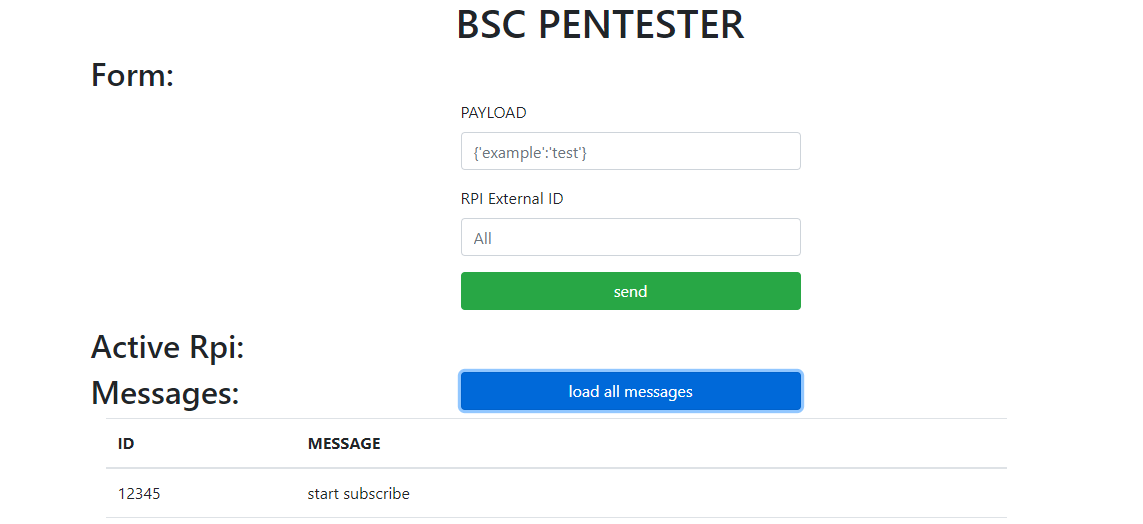
\includegraphics[width=\textwidth]{gui2}
    \caption{Prezentacja zaimplementowanego interfejsu użytkownika}
    \label{fig:gui2}
\end{figure}